\begin{frame}{Research Plan}
    \begin{itemize}
        \item Explicit (e.g., CBBA) and implicit methods for decentralized MRTA face challenges with dynamic environments
        \begin{itemize}
            \item Explicit methods only allow robots to use local information 
            % \item Standard consensus approaches in implicit methods lead to large errors 
            \pause
            \item Standard consensus in implicit methods lead to zero steady-state error but leads to large errors when the information is changing
        \end{itemize}     
        \begin{equation*}
            \label{standard method}
            \hat{z}_{i,d}[k+1] =  \hat{z}_{i,d}[k] + \gamma \mu_{i,d}[k],   \quad \text{with} \quad \mu_{i,d}[k] = \sum_{j \in \mathcal{N}_i} w_{i,j}\left(\hat{z}_{j,d}[k] - \hat{z}_{i,d}[k]\right).
        \end{equation*}
        \vspace{-0.6cm}
        \visible<2>{
        \begin{figure}[H] 
            \centering
                \subfloat[\label{Fig_standard_1}Standard consensus]{%
               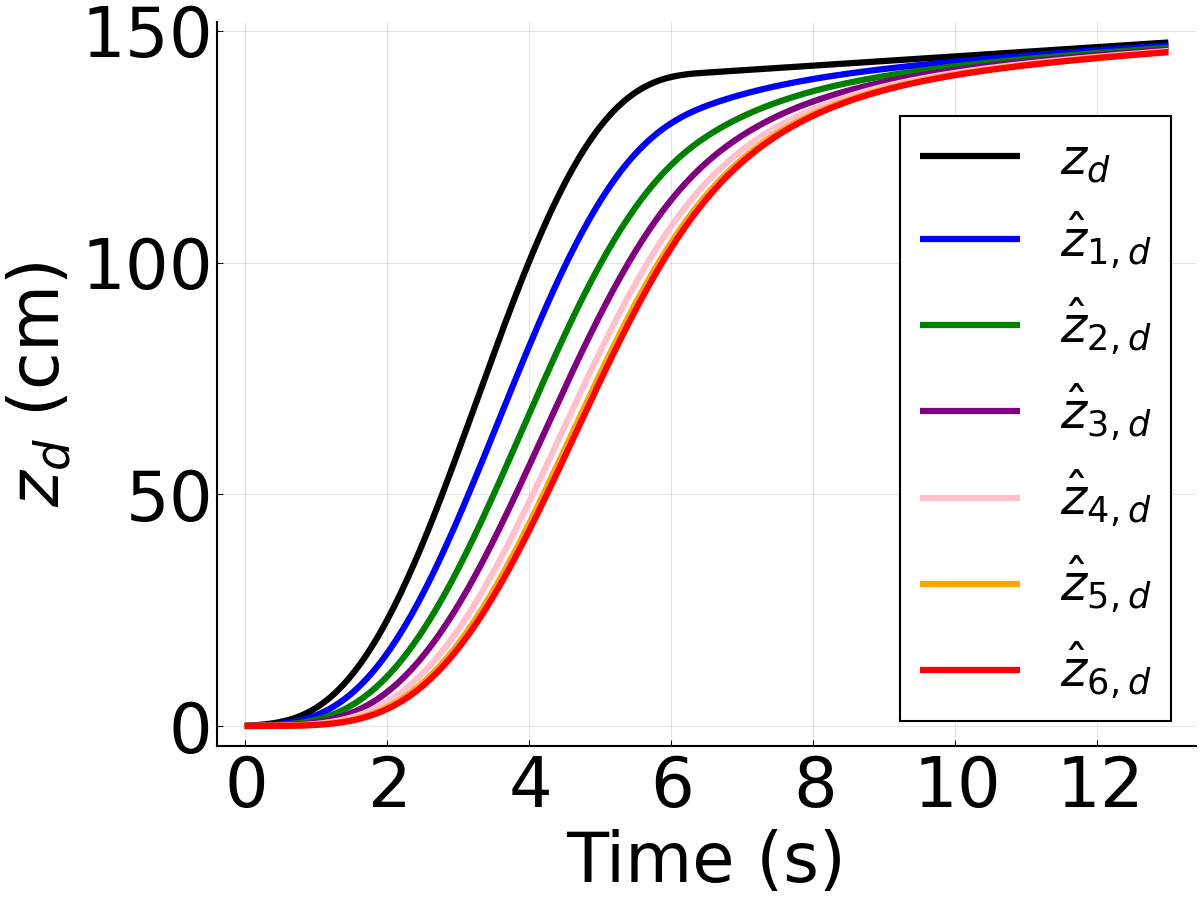
\includegraphics[width=0.4\linewidth]{Figures/standard_quals.png}}

           \subfloat[\label{Communication_network_1}Communication network]{
            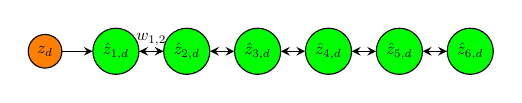
\begin{tikzpicture}[>=stealth, scale=0.6, transform shape] % Stealth arrow tips
              % First node (special)
              \node[draw, circle, fill=orange] (zd) at (0,0) {$z_d$};
              
              % Other nodes
              \foreach \x in {1,...,6}
                \node[draw, circle, fill=green, text=black] (\x) at (\x*1.5,0) {$\hat{z}_{\x,d}$};
              
              % Directed edge from zd to 1
              \draw[->] (zd) -- (1);
              
              % Undirected edges from 1 to 6
              \foreach \x [remember=\x as \lastx (initially 1)] in {2,...,6}
                \draw[<->] (\lastx) -- (\x);

            \draw (1) -- node[above] {$w_{1,2}$} (2);
            \end{tikzpicture}

            }
        \end{figure}}
    \end{itemize}
\end{frame}

% \begin{frame}{Research Plan}
%     \begin{itemize}
%         \item Dynamic MRTA in time-varying environments
%         \item Environment is changing and uncertain (e.g., wildfire tracking/management and search and rescue operations) 
%         \begin{itemize}
%             \item Unknown dynamics
%             \item Partial observability
%         \end{itemize}
%          % \item Wildfire tracking and management application: drones collect atmospheric measurements on the canopy of the wildfire and provide a real-time fire spread prediction model~\cite{DronesWildfire}.
%     \end{itemize}
   
%     \begin{figure}
%         \centering
%         \subfloat[~\cite{DronesWildfire,chen2024drone}]
%         {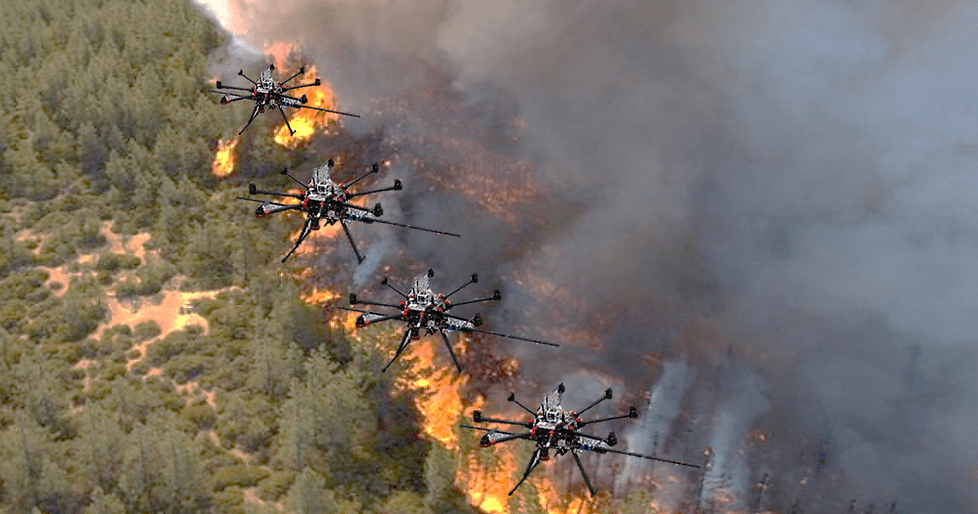
\includegraphics[width=0.5\linewidth]{Figures/Drones-and-wildfire.png}}
%     \end{figure}
% \end{frame}

\begin{frame}{Research Plan}
    \begin{itemize}
        \item Improve the accuracy of the information communicated using delayed-self reinforcement (DSR)~\cite{devasia2020cohesive}
    \end{itemize}
    \begin{equation*}
        \label{dsr method}
        \hat{z}_{i,d}[k+1] =  \underbrace{\hat{z}_{i,d}[k] + \gamma \mu_{i,d}[k]}_{\text{standard method}} + \underbrace{\beta_1 \left(\mu_{i,d}[k] - \mu_{i,d}[k-1]\right) + \beta_2 \left(\hat{z}_{i,d}[k] - \hat{z}_{i,d}[k-1]\right)}_{\text{DSR terms}}.
    \end{equation*}
    \vspace{-0.6cm}
    \begin{figure}[H] 
    \centering
    \subfloat[\label{Fig_standard}Standard consensus]{%
       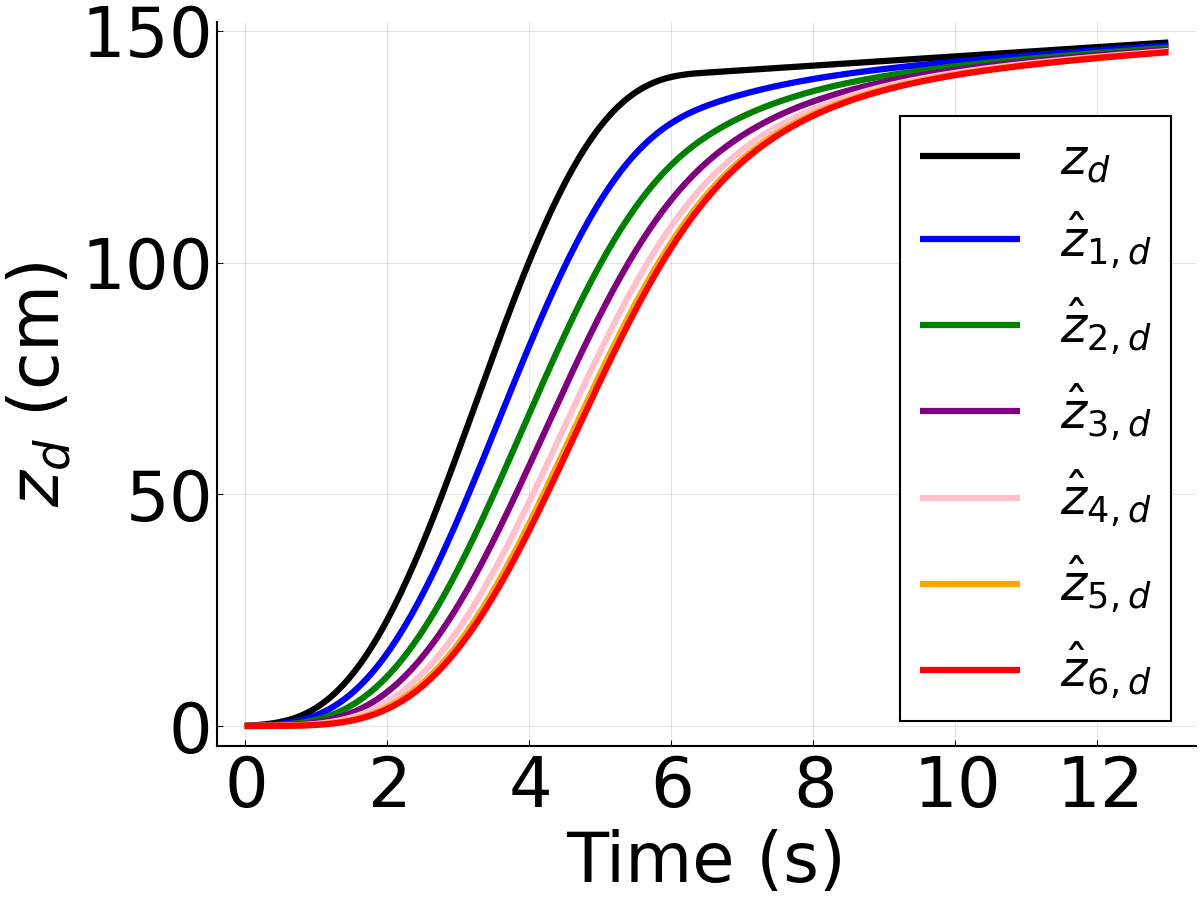
\includegraphics[width=0.42\linewidth]{Figures/standard_quals.png}}
    \hfill
    \subfloat[\label{Fig_dsr}DSR]{%
        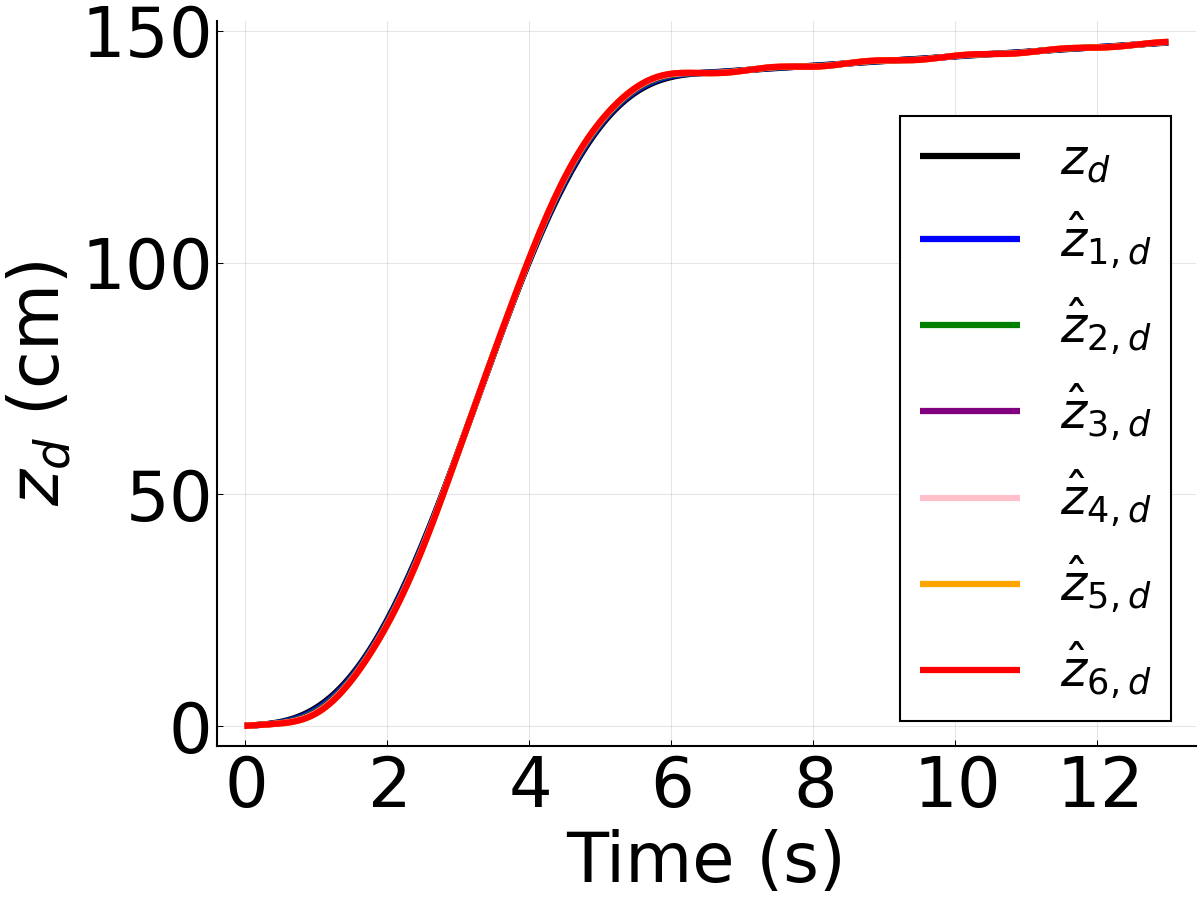
\includegraphics[width=0.42\linewidth]{Figures/dsr_quals.png}}
  \label{Fig_sims} 
\end{figure}
\begin{itemize}
    % \item Potential improvement in decision-making for the dynamic MRTA
    \item Potential improvement for decision-making in time-critical MRTA
\end{itemize}
\end{frame}

\begin{frame}{Research Directions}
    Decentralized decision-making methods for networked systems in dynamic environments
    \begin{columns}
    \begin{column}{0.65\textwidth}
        \begin{enumerate}
        \addtolength{\itemindent}{0.5cm}
        \item Can accurate information communication be maintained in volatile environments?
        \begin{itemize}
            \item Potential approach: Higher-order DSR for communicating information with higher-order dynamics
        \end{itemize}
        \pause
        \item How can learning approaches be utilized to solve dynamic decentralized MRTA problems?
        \begin{itemize}
            \item Current methods treat MRTA problems as static optimization problems and replan each time step.
            \item Potential approach: develop learned policies using multi-agent reinforcement learning by approximating dynamic MRTA problems (lookahead/rollout-based optimization~\cite{bhattacharya2021multiagent}).
            \item Accurate information communication needed for the decentralized policies and modeling   
        \end{itemize}
        \end{enumerate}
        \end{column}
        \begin{column}{0.5\textwidth}
            \includemovie[attach=false,autoplay,text={%
            % 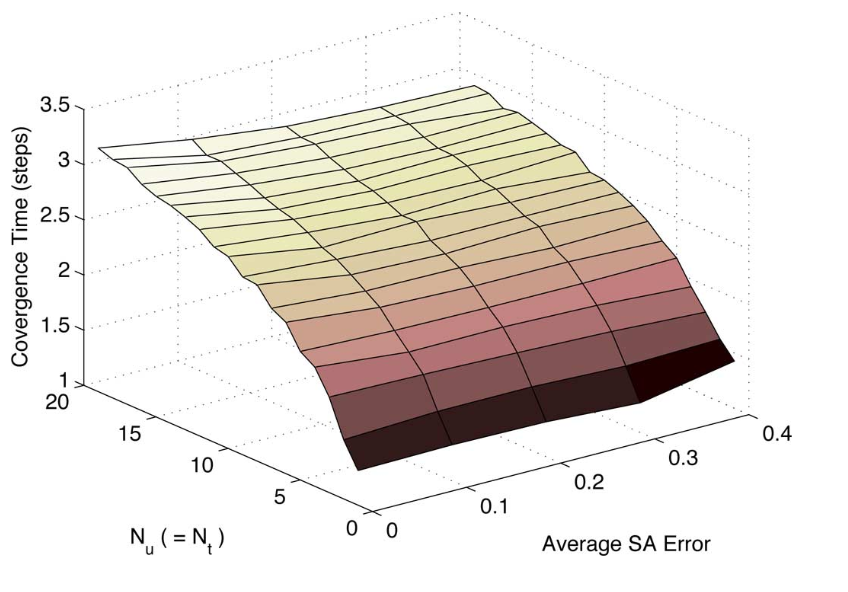
\includegraphics{Figures/convergence_time.png}%
            }]{1.0\linewidth}{1.0\linewidth}{drone_wildfire.gif}
        \end{column}
    \end{columns}
        % \item However, to incorporate dynamics and to account for the rapidly changing environment, I will explore learning methods for policies to general MRTA problems.
        % \item Additionally, I will investigate how DSR can be utilized in the learning process to offer faster learning rates and better policies.
        
        % \item Decentralized networked multi-agent reinforcement learning (MARL) where online policy learning relies on the state of the environment 
\end{frame}

% \begin{frame}
%   \begin{center}
%     \includemovie[attach=false,autoplay,text={%
%         % 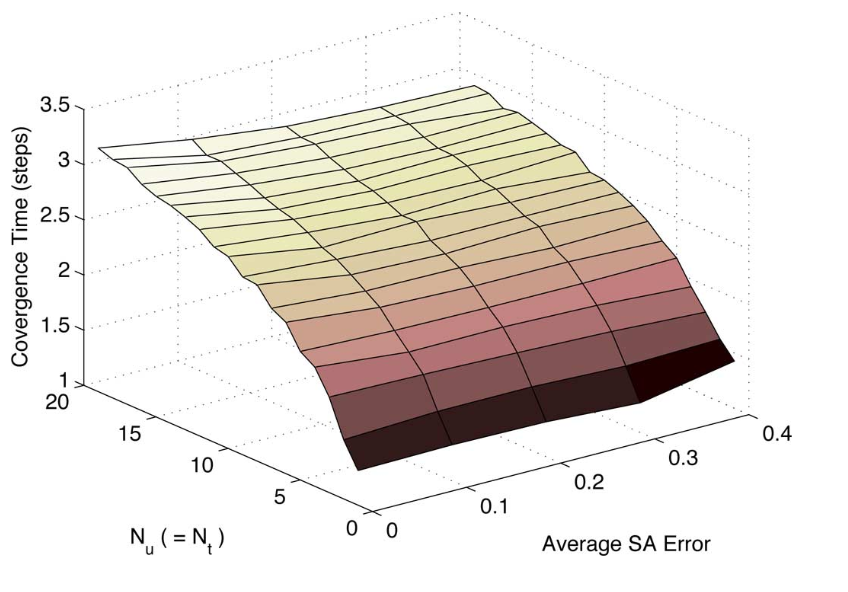
\includegraphics{Figures/convergence_time.png}%
%       }]{1.0\linewidth}{1.0\linewidth}{drone_wildfire.gif}
%   \end{center}
% \end{frame}

\begin{frame}
    \frametitle{Summary}
    \textbf{Presentation content:}
    \begin{itemize}
        \item Literature Review
        \item Paper Review
        \item Research Plan
    \end{itemize}

    \vspace{1cm}
    \textbf{Committee:}
    \begin{itemize}
        \item \textbf{Santosh Devasia} | Faculty Advisor
        \item \textbf{Junlan Wang} | Departmental Representative
        \item \textbf{Xu Chen} | Committee Member
        \item \textbf{Shuonan Dong} | Committee Member
    \end{itemize}

    \vspace{1cm}
    \centering
    \Huge{Questions?}
\end{frame}
